\documentclass[a4paper,twoside]{report}

%%% change the year here
\newcommand{\rtbyear}{2020}

\usepackage{times}
\usepackage{graphicx}
\usepackage{wrapfig}
\usepackage{pdfpages}
\usepackage{hyperref}
\usepackage{fancyhdr}
\usepackage[overlay]{textpos}
% fonts
\usepackage{mathptmx}
\usepackage{anyfontsize}
\usepackage{amsfonts}  % mathbb font
\usepackage{textcomp}     % access \textquotesingle
\usepackage{t1enc}
\usepackage{fancyvrb}
\fvset{formatcom=\color{blue},fontseries=c,fontfamily=courier,xleftmargin=4mm,commentchar=!}

% other
\usepackage{booktabs,longtable}
\hypersetup{
  colorlinks=true,
  linkcolor=black
  }
  
\def\topfraction{.9}
\def\bottomfraction{.9}
\def\textfraction{.1}
\def\floatpagefraction{.9}

\setlength{\parindent}{0mm}
\usepackage{parskip}
\usepackage{color}
\usepackage{sectsty}
\allsectionsfont{\sffamily}
\makeatletter
\newcommand\funcsection{%
\@startsection{section}{1}{\z@}%
  {-3.5ex \@plus -1ex \@minus -.2ex}%
  {2.3ex \@plus.2ex}%
  {\color{red}\sffamily\huge\bfseries}}
\makeatother

\input{release.tex}

%\usepackage{multind}
\usepackage{multicol}

% printindex stuff

\makeatletter
\def\printindex#1#2{\subsection*{#2}
  \@input{#1.ind}}
  
\def\theindex{\parindent\z@
\parskip\z@ plus .3pt\relax\let\item\@idxitem}
\def\@idxitem{\par\hangindent 40pt}
\def\subitem{\par\hangindent 40pt \hspace*{20pt}}
\def\subsubitem{\par\hangindent 40pt \hspace*{30pt}}
\def\endtheindex{}
\def\indexspace{\par \vskip 10pt plus 5pt minus 3pt\relax}
\makeatother

\DefineVerbatimEnvironment{Code}{Verbatim}{formatcom=\color{blue},fontseries=c,fontfamily=courier,fontsize=\footnotesize,xleftmargin=4mm,commentchar=!}
\pagestyle{empty}

\def\Mlab{MATLAB}

\begin{document}
\setlength{\TPHorizModule}{1cm}
\setlength{\TPVertModule}{1cm}

%%%%%%%%%%%%%%%%% TITLE PAGE
\begin{textblock}{19}(-3.5,-4.5)
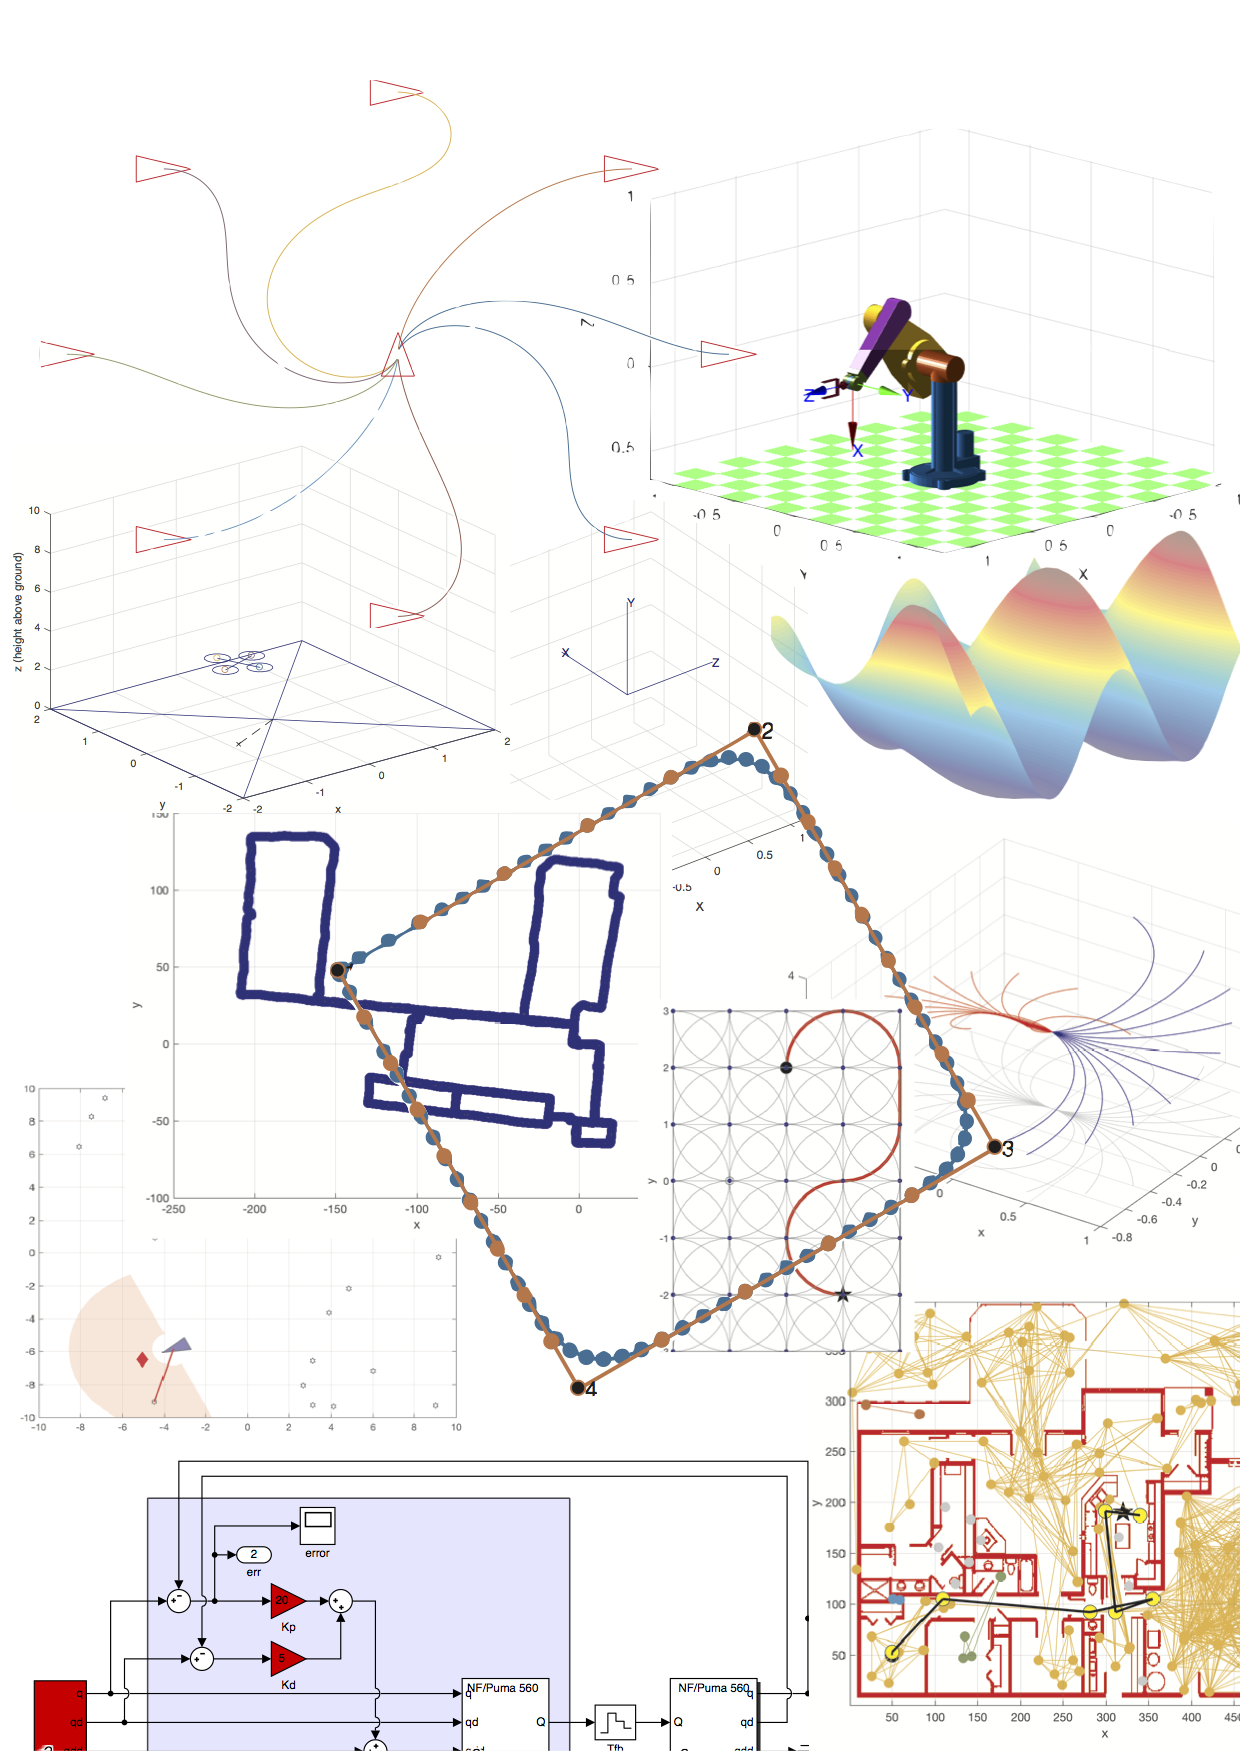
\includepdf{titlepage}
\fontsize{75}{80}\selectfont
\textbf{Robotics Toolbox}\\[5pt]
\fontsize{40}{45}\selectfont
for MATLAB\textsuperscript{\textregistered}\\[5pt]
Release 10

\vspace*{20.5cm}
\hfill\textbf{Peter Corke}\\[5pt]
\end{textblock}
\thispagestyle{empty}
\newpage
%%%%%%%%%%%%%%%%% INSIDE FRONT COVER
\vspace*{\fill}
\begin{tabular}{ll}
Release & \release \\
Release date & \reldate \\[20pt]
Licence & LGPL \\
Toolbox home page &  \url{http://www.petercorke.com/robot} \\
Discussion group & \url{http://groups.google.com.au/group/robotics-tool-box}
\end{tabular}
\vspace*{\fill}
\hrule
Copyright \textcopyright \rtbyear Peter Corke\\
peter.i.corke$@$gmail.com\\
\url{http://www.petercorke.com}
\vspace*{\fill}
\setlength{\fboxsep}{10pt}%

%%%%%%%%%%%%%%%% CONTENT
\pagestyle{headings}        % Gives page headings at top of page
\lfoot{Robotics Toolbox \release\ for \Mlab\textsuperscript{\textregistered} }
\rfoot{Copyright \copyright Peter Corke \rtbyear}

\setcounter{section}{0}
\addcontentsline{toc}{section}{Preface}
\chapter*{Preface}
\pagestyle{fancyplain}
\begin{wrapfigure}{l}{4cm}
\vspace{-2ex}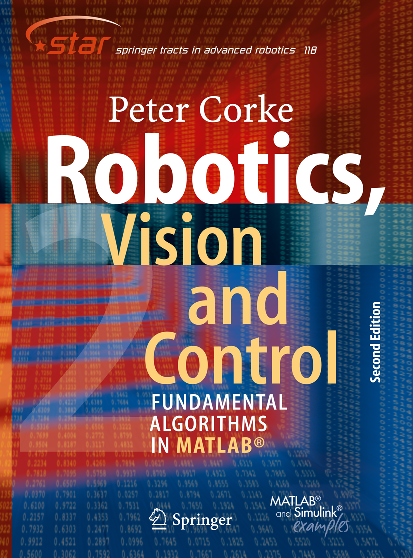
\includegraphics[width=3.5cm]{figs/frontcover.pdf}
\end{wrapfigure}
This, the tenth major release of the Toolbox, representing over twenty five years of continuous
development and a substantial level of maturity.
This version corresponds to the \textbf{second edition} of the book ``\textit{Robotics, Vision \& Control}'' published in June 2017 -- RVC2.

This \Mlab\textsuperscript{\textregistered} Toolbox has a rich collection of functions that are useful for the study and simulation
of robots:  arm-type robot manipulators and mobile robots.
For robot manipulators, functions include kinematics, trajectory generation, dynamics and  control.
For mobile robots, functions include path planning, kinodynamic planning, 
localization, map building and simultaneous localization and mapping (SLAM).

The Toolbox makes strong use of classes to represent robots and such things as sensors and maps.
It includes Simulink\textsuperscript{\textregistered} models to describe the evolution of arm or mobile robot state over time for a number of classical control
strategies. The Toolbox also provides functions for manipulating and converting between datatypes such as vectors, rotation matrices, unit-quaternions, quaternions, homogeneous transformations and twists which are necessary to represent  position and orientation in 2- and
3-dimensions.

The code is written in a straightforward manner which allows
for easy understanding, perhaps at the expense of computational efficiency.
If you feel strongly about computational efficiency then you can always
rewrite the function to be more efficient,
compile the M-file using the \Mlab\   compiler, or
create a MEX version.

The bulk of this manual is auto-generated from the comments in the \Mlab\ code itself.
For elaboration on the underlying principles, extensive illustrations and worked examples please consult
 ``\textit{Robotics, Vision \& Control, second edition}''  which provides a detailed discussion (720 pages, nearly 500 figures and over 1000 code examples) of how to use the Toolbox functions to solve many types of problems in robotics.


\cleardoublepage
\chapter*{Functions by category}
\addcontentsline{toc}{section}{Functions by category}
\begin{multicols}{2}
\IfFileExists{funcidx_body.tex}{\input{funcidx_body.tex}}{} 
\end{multicols}

\cleardoublepage
\tableofcontents

\newpage
\chapter{Introduction}

\section{Changes in RTB 10}
RTB 10 is largely backward compatible with RTB 9.

\subsection{Incompatible changes}

\begin{itemize}
\item The class \texttt{Vehicle} no longer represents an Ackerman/bicycle vehicle model.  \texttt{Vehicle} is now an abstract superclass of \texttt{Bicycle} and \texttt{Unicycle} which represent car-like and differentially-steered vehicles respectively.
\item The class \texttt{LandmarkMap} replaces \texttt{PointMap}.
\item Robot-arm forward kinematics now returns an \texttt{SE3} object rather than a $4\times4$ matrix.
\item The \texttt{Quaternion} class used to represent both unit and non-unit quaternions which was untidy and confusing.  They are now represented by two classes \texttt{UnitQuaternion} and \texttt{Quaternion}.
\item The method to compute the arm-robot Jacobian in the end-effector frame has been renamed from \texttt{jacobn} to \texttt{jacobe}.
\item The path planners, subclasses of \texttt{Navigation}, the method to find a path has been renamed from \texttt{path} to  \texttt{query}.
\item The Jacobian methods for the \texttt{RangeBearingSensor} class have been renamed to \texttt{Hx}, \texttt{Hp}, \texttt{Hw}, \texttt{Gx},\texttt{Gz}.
\item The function \texttt{se2} has been replaced with the class \texttt{SE2}.  On some platforms (Mac) this is the same file.  Broadly similar in function, the former returns a $3\times 3$ matrix, the latter returns an object.
\item The function \texttt{se3} has been replaced with the class \texttt{SE3}.  On some platforms (Mac) this is the same file.  Broadly similar in function, the former returns a $4\times 4$ matrix, the latter returns an object.
\end{itemize}

These changes are summarized in Table \ref{tab:changes}.

\begin{table}
\centering
\begin{tabular}{|l|l|}\hline
\textbf{RTB 9} & \textbf{RTB 10} \\ \hline\hline
\texttt{Vehicle} & \texttt{Bicycle}\\
\texttt{Map} & \texttt{LandmarkMap} \\
\texttt{jacobn} & \texttt{jacobe} \\
\texttt{path} & \texttt{query} \\
\texttt{H\_x} & \texttt{Hx} \\
\texttt{H\_xf} & \texttt{Hp} \\
\texttt{H\_w} & \texttt{Hw} \\
\texttt{G\_x} & \texttt{Gx} \\
\texttt{G\_z} & \texttt{Gz} \\ \hline
\end{tabular}
\caption{Function and method name changes}\label{tab:changes}
\end{table}

\subsection{New features}
\begin{itemize}
\item \texttt{SerialLinkplot3d()} renders realistic looking 3D models of robots.   STL models from
 the package ARTE by Arturo Gil (\url{https://arvc.umh.es/arte}) are now included with RTB, by kind permission.
\item \texttt{ETS2} and \texttt{ETS3} packages provide a gentle (non Denavit-Hartenberg) introduction to robot arm kinematics, see Chapter 7 for details.
\item Distribution as an \texttt{.mltbx} format file.
\item A comprehensive set of functions to handle rotations and transformations in 2D, these functions end with the suffix 2, eg. \texttt{transl2}, \texttt{rot2}, \texttt{trot2} etc.
\item Matrix exponentials are handled by \texttt{trexp}, \texttt{trlog}, \texttt{trexp2} and \texttt{trlog2}.
\item The class \texttt{Twist} represents a twist in 3D or 2D.  Respectively, it is a 6-vector representation of the Lie algebra $se(3)$, or a
3-vector representation of $se(2)$.
\item The method \texttt{SerialLink.jointdynamics} returns a vector of \texttt{tf} objects representing the dynamics of the joint actuators.
\item The class \texttt{Lattice} is a simple kino-dynamic lattice path planner.
\item The class \texttt{PoseGraph} solves graph relaxation problems and can be used for bundle adjustment and pose graph SLAM.
\item The class \texttt{Plucker} represents a line using Pl\'{u}cker coordinates.
\item The folder \texttt{RST} contains Live Scripts that demonstrate some capabilities of the MATLAB Robotics System Toolbox\textsuperscript{TM}.
\item The folder \texttt{symbolic} contains Live Scripts that demonstrate use of the MATLAB Symbolic Math Toolbox\textsuperscript{TM}
for deriving Jacobians used in EKF SLAM (vehicle and sensor), inverse kinematics for a 2-joint planar arm and solving for roll-pitch-yaw angles
given a rotation matrix.
\item All the robot models, prefixed by \texttt{mdl\_}, now reside in the folder \texttt{models}.
\item New robot models include Universal Robotics UR3, UR5 and UR10; and Kuka light weight robot arm.
\item A new folder \texttt{data} now holds various data files as used by examples in RVC2: STL models, occupancy grids, Hershey font, Toro and G2O
data files.
\end{itemize}

Since its inception RTB has used matrices\footnote{Early versions of RTB, before 1999, used vectors to represent quaternions but that changed to an object once objects were added to the language.} to represent rotations and transformations in 2D and 3D.  A trajectory, or sequence, was represented by a 3-dimensional matrix, eg. $4\times 4 \times N$.  In RTB10 a set of classes have been introduced to represent orientation and pose in 2D and 3D: \texttt{SO2}, \texttt{SE2}, \texttt{SO3}, \texttt{SE3}, \texttt{Twist} and \texttt{UnitQuaternion}.  These classes are fairly polymorphic, that is, they share many methods and operators\footnote{For example, you could substitute objects of class \texttt{SO3} and \texttt{UnitQuaternion} with minimal code change.}.  All have a number of static methods that serve as constructors from particular representations.  A trajectory is represented by a vector of these objects which makes code easier to read and
understand.  Overloaded operators are used so the classes behave in a similar way to native matrices\footnote{The capability is extended so that we can element-wise multiple two vectors of transforms, multiply one transform over a vector of transforms or a set of points.}.
The relationship between the classical Toolbox functions and the new classes are shown in Fig \ref{fig:newfunctions}.

You can continue to use the classical functions.  The new classes have methods with the names of classical functions to provide similar functionality.  For instance
\begin{Code}
>> T = transl(1,2,3);  % create a 4x4 matrix
>> trprint(T)  % invoke the function trprint
>> T = SE3(1,2,3);  % create an SE3 object
>> trprint(T)  % invoke the method trprint
>> T.T   % the equivalent 4x4 matrix
>> double(T) % the equivalent 4x4 matrix
\end{Code}

\begin{Code}
>> T = SE3(1,2,3);  % create a pure translation SE3 object
>> T2 = T*T;  % the result is an SE3 object
>> T3 = trinterp(T, T2,, 5); % create a vector of five SE3 objects between T and T2
>> T3(1)  % the first element of the vector
>> T3*T  % each element of T3 multiplies T, giving a vector of five SE3 objects
\end{Code}

\begin{figure}[p]
\centering
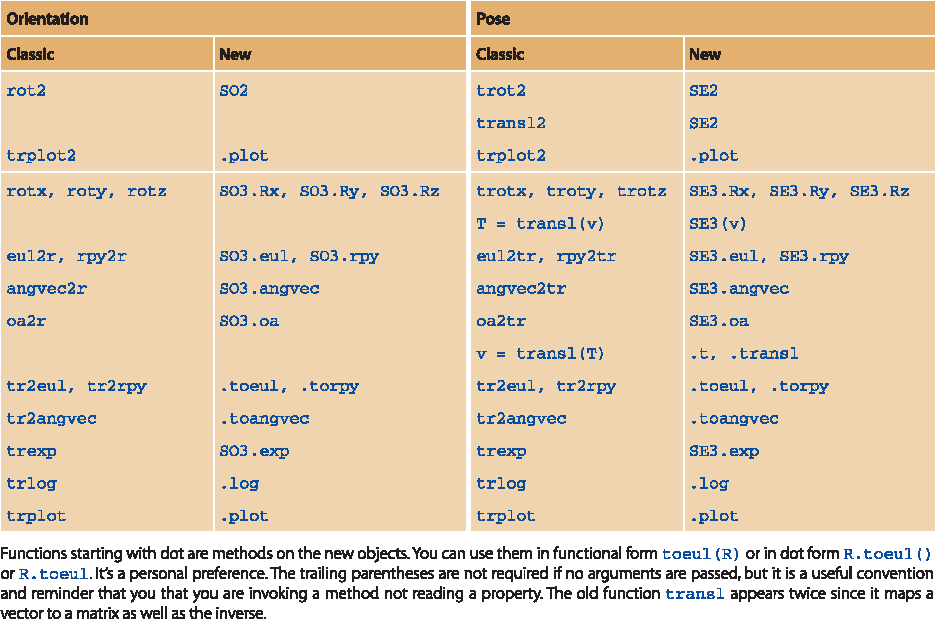
\includegraphics[width=\textwidth]{figs/CT-02-03.pdf}
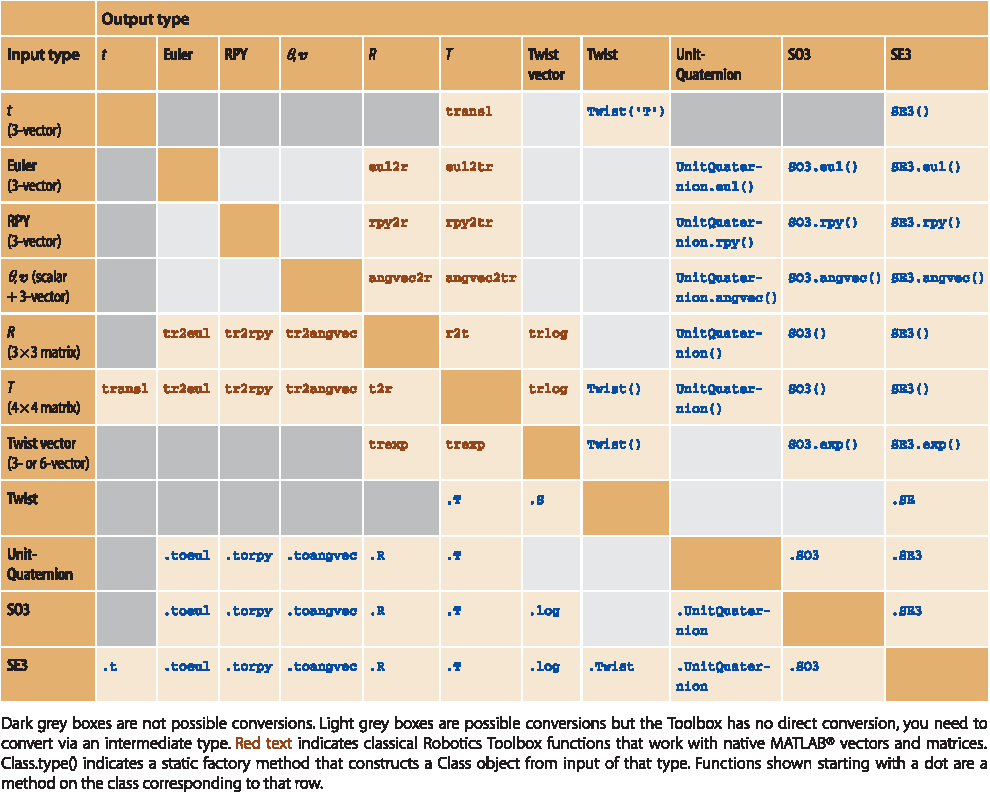
\includegraphics[width=\textwidth]{figs/CT-02-02.pdf}
\caption{(top) new and classic methods for representing orientation and pose, (bottom) functions and methods to convert
between representations.  Reproduced from ``\textit{Robotics, Vision \& Control, second edition, 2017}''}\label{fig:newfunctions}
\end{figure}

\subsection{Enhancements}
\begin{itemize}
\item Dependencies on the Machine Vision Toolbox for MATLAB (MVTB) have been removed.  The fast dilation function used for path planning is now searched for in MVTB and the MATLAB Image Processing Toolbox (IPT) and defaults to a provided M-function.
\item A major pass over all code and method/function/class documentation.
\item Reworking and refactoring all the manipulator graphics, work in progress.
%\item Some file system changes: all robot models in the folder \texttt{models} and various data files aggregated into the folder \texttt{data}.
%\item Two ``apps'' are included: \texttt{tripleangle} and \texttt{configspace}.
\item An ``app" is included: \texttt{tripleangle} which allows graphical experimentation with Euler and roll-pitch-yaw angles.
\item A tidyup of all Simulink models.  Red blocks now represent user settable parameters, and shaded boxes are used to group parts of the models.
\item RangeBearingSensor animation
\item All the java code that supports the \texttt{DHFactor} functionality now lives in the folder \texttt{java}.  The \texttt{Makefile} in there can be used
to recompile the code.  There are java version issues and the shipped class files are built to java 1.7 which allows operation
\end{itemize}

\section{Changes in RTB 10.3}
\begin{figure}[b]
\centering
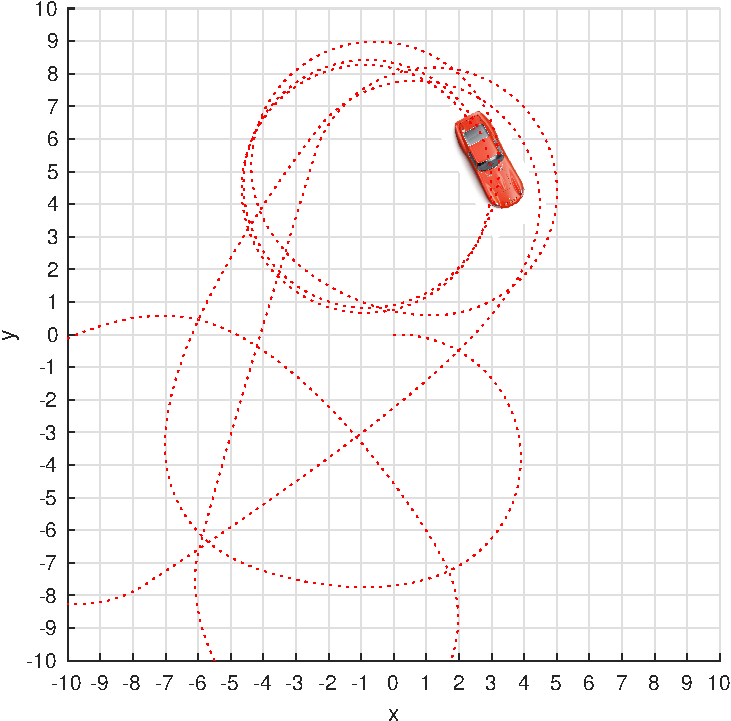
\includegraphics[width=6cm]{figs/caranim.pdf} 
\caption{Car animation drawn with \texttt{demos/car\_anim} using \texttt{plot\_vehicle}}\label{fig:caranim}
\end{figure}

This release includes minor new features and  a number of bug fixes compared to 10.2:
\begin{itemize}
\item Serial-link manipulators
    \begin{itemize}
    \item The Symbolic Robot Modeling Toolbox component by J\"{o}rn Malzahn has been updated.  It offers amazing speedups by using symbolic algebra to create robot specific MATLAB code or MEX files and it can even generate optimised Simulink blocks.  I've seen speedups of over 50,000x.  You need to have the Symbolic Math Toolbox.
    \item New robot kinematic models: Franka-Emika PANDA and Rethink Sawyer.
    \item Methods \texttt{DH} and \texttt{MDH} on the \texttt{SerialLink} class convert models between DH and MDH kinematics. Dynamics not yet supported.
    \item \texttt{plot3d} behaves like \texttt{plot} for the \texttt{'trail'} and \texttt{'movie'} options.
    \item Experimental feature: Manipulator configuration (joint angle) vectors can be kept \textit{inside} the \texttt{SerialLink} object.  At constructor time
    	the option \texttt{'configs', \{'qz', qz, 'qr', qr\}} adds these two configurations to the class instance, and they can be referenced later as, for 	example, \texttt{p560.qz}.  This reduces the number of workspace variables and confusion when working with several robots at the same 	time.
	
\item Fix bug in the \texttt{'trail'} option for \texttt{SerialLink.plot}.

\item Fixed bug in \texttt{ikunc}, \texttt{ikcon} which ignored \texttt{q0}.
    \end{itemize}
\item Mobile robotics
\begin{itemize}
\item Added the ability to animate a picture of a vehicle to \texttt{plot\_vehicle}, see \texttt{demos/car\_demo} and Figure \ref{fig:caranim}.  Also added a \texttt{'trail'} feature, and updated documentation.
	\item Experimental feature : A Reeds-Shepp path planner, see \texttt{rReedsShepp.m} and \texttt{demos/reedsshepp.mlx}, this is not (yet) properly integrated
	into the \texttt{Navigation} class architecture.
\end{itemize}

\item Simulink
\begin{itemize}
\item Simulink blocks for Euler angles now have a checkbox to allow degrees mode.
\item Simulink blocks for roll-pitch-yaw angles now have a checkbox to allow degrees mode and radio buttons to select the angle sequence.
\item New Simulink block for \texttt{mstraj} gives full access to all capabilities of that function.
\item A folder \texttt{simulink/R2015a} contains all the Simulink models exported as \texttt{.slx} files for Simulink R2015a.  This might
ease problems for those using older versions of Simulink on the models in the top folder, many of which have been edited and saved
under R2018a.  Check the README file for details.


\end{itemize}

\item A new script \texttt{rvccheck} which attempts to diagnose installation and MATLAB path issues.
\item The \texttt{demos} folder now includes  LiveScript versions of  each demo, these are \texttt{.mlx} files.
  I've done a first pass at formatting the content and in a few cases updating the content a little.  From here on, the \texttt{.m} files are 
  deprecated.  You need MATLAB 2016a or later to run the LiveScripts.
\item Major tidyup and documentation improvements for the \texttt{Twist} and \texttt{Plucker} objects.

\item Changes to the \texttt{RTBPose.mtimes} method which now allows you to:
\begin{itemize}
	\item postmultiply an \texttt{SE3} object by a \texttt{Plucker} object which returns a \texttt{Plucker} object.  This applies a rigid-body transformation to the line in space.
	\item postmultiply an \texttt{SE2} object by a MATLAB \texttt{polyshape} object which returns a  \texttt{polyshape} object.  This applies a rigid-body transformation to the polygon.
\end{itemize}
\item  Added a \texttt{disp} method to various toolbox objects, invokes \texttt{display}, which provides a display of the type from within the  debugger.

\item \texttt{Quaternion} \texttt{==} operator
\item  \texttt{UnitQuaternion}  \texttt{==}  accounts for double mapping
\item \texttt{UnitQuaternion} has a \texttt{rand} method that generates a randomly distributed rotation,  also used by \texttt{SO3.rand} and  \texttt{SE3.rand}.
\item \texttt{tr2rpy} fixed a long standing bug with the pitch angle in certain corner cases, the pitch angle now lies in the range $[-\pi, \,+\pi)$.

\item Remove dependency on \texttt{numrows()} and \texttt{numcols()} for \texttt{rt2tr}, \texttt{tr2rt}, \texttt{transl}, \texttt{transl2} which simplifies standalone operation.

\item A campaign to reduce the size of the RTB distribution file:
\begin{itemize}
	\item \texttt{tripleangle} uses updated STL files with reduced triangle counts for faster loading.
	\item This manual is compressed.
	\item Removal of extraneous files.
\end{itemize}
\begin{wrapfigure}{l}{4cm}
\vspace{-2ex}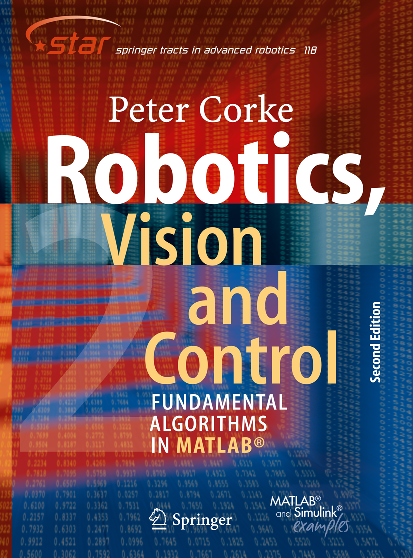
\includegraphics[width=3.5cm]{figs/frontcover.pdf}
\end{wrapfigure}

\item Options to RTB functions can now be strings or character arrays, ie. \texttt{rotx(45, 'deg')} or \texttt{rotx(45, "deg")}.  If you don't yet know about MATLAB strings (with double quotes) check them out.
\item General tidyup to code and documentation, added missing files from earlier releases.
\end{itemize}

\section{Changes in RTB 10.2}
This release has a relatively small number of bug fixes compared to 10.1:
\begin{itemize}
\item Fixed bugs in \texttt{jacobe} and \texttt{coriolis} when using symbolic arguments.
\item New robot models: UR3, UR5, UR10, LWR.
\item Fixed bug for \texttt{interp} method of \texttt{SE3} object.
\item Fixed bug with detecting Optimisation Toolbox for \texttt{ikcon} and \texttt{ikunc}.
\item Fixed bug in \texttt{ikine\_sym}.
\item Fixed various bugs related to plotting robots with prismatic joints.
\end{itemize}


\section{How to obtain the Toolbox}
The Robotics Toolbox is freely available from the Toolbox home
page at 
\begin{quote}
\url{http://www.petercorke.com}
\end{quote}

%The web page requests some information from you
%regarding such as your country, type of organization and application.
%This is just a means for me to gauge interest and to remind myself
%that this is a worthwhile activity.

The file is available in \Mlab toolbox format (\texttt{.mltbx}) or zip format (\texttt{.zip}). 

\subsection{From .mltbx file}
Since MATLAB R2014b toolboxes can be packaged as, and installed from, files with the extension \texttt{.mltbx}. Download the most recent version of \texttt{robot.mltbx} or \texttt{vision.mltbx} to your computer. Using MATLAB navigate to the folder where you downloaded the file and double-click it (or right-click then select Install). The Toolbox will be installed within the local MATLAB file structure, and the paths will be appropriately configured for this, and future MATLAB sessions.

\subsection{From .zip file}
Download the most recent version of robot.zip or vision.zip to your computer. Use your favourite unarchiving tool to unzip the files that you downloaded.
To add the Toolboxes to your MATLAB path execute the command
\begin{verbatim}
  >> addpath RVCDIR ;
  >> startup_rvc
\end{verbatim}
where \texttt{RVCDIR} is the full pathname of the folder where the folder \texttt{rvctools} was created when you unzipped the Toolbox files. The script \texttt{startup\_rvc} adds various subfolders to your path and displays the version of the Toolboxes.
After installation the files for both Toolboxes reside in a top-level folder called \texttt{rvctools} and beneath this are a number of folders:

\begin{tabular}{ll}
\texttt{robot} & The Robotics Toolbox \\
\texttt{vision} & The Machine Vision Toolbox\\
\texttt{common} & Utility functions common to the Robotics and Machine Vision Toolboxes\\
\texttt{simulink}  & Simulink blocks for robotics and vision, as well as examples \\
\texttt{contrib} & Code written by third-parties\\
\end{tabular}

If you already have the Machine Vision Toolbox installed then download
the zip file to the folder above the existing \texttt{rvctools} directory,
and then unzip it.
The files from this zip archive will properly interleave with the Machine
Vision Toolbox files.

You need to setup the path every time you start \Mlab\ but you can 
automate this by setting up environment variables, editing your 
\texttt{startup.m} script, using \texttt{pathtool} and saving the path, or by pressing the ``Update Toolbox Path
Cache" button under \Mlab\ General preferences.
You can check the path using the command \texttt{path} or \texttt{pathtool}.

A menu-driven demonstration can be invoked by 
\begin{verbatim}
  >> rtbdemo
\end{verbatim}


\subsection{MATLAB Online\textsuperscript{TM}}
The Toolbox works well with MATLAB Online\textsuperscript{TM} which lets you access a \Mlab\ session from a web browser, tablet 
or even a phone.
The key is to get the RTB files into the filesystem associated with your Online account.  The easiest way to do this is to install
MATLAB Drive\textsuperscript{TM} from MATLAB File Exchange or using the Get Add-Ons option from the MATLAB GUI.  This functions
just like Google Drive or Dropbox, a local filesystem on your computer is synchronized with your MATLAB Online account.  Copy the RTB
files into the local MATLAB Drive cache and they will soon be synchronized, invoke \texttt{startup\_rvc} to setup the paths and you are ready to simulate robots on your mobile device or in a web browser.

\subsection{Simulink\textsuperscript{\textregistered}}
\begin{figure}
\begin{tabular}{cc}
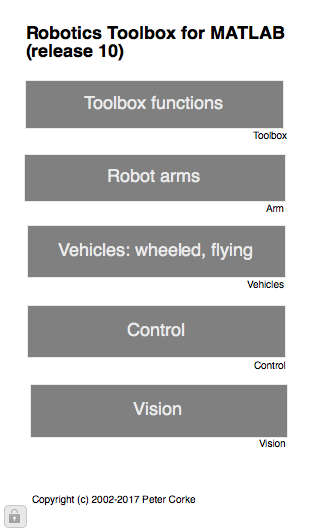
\includegraphics[width=6cm]{figs/roblocks.png} & 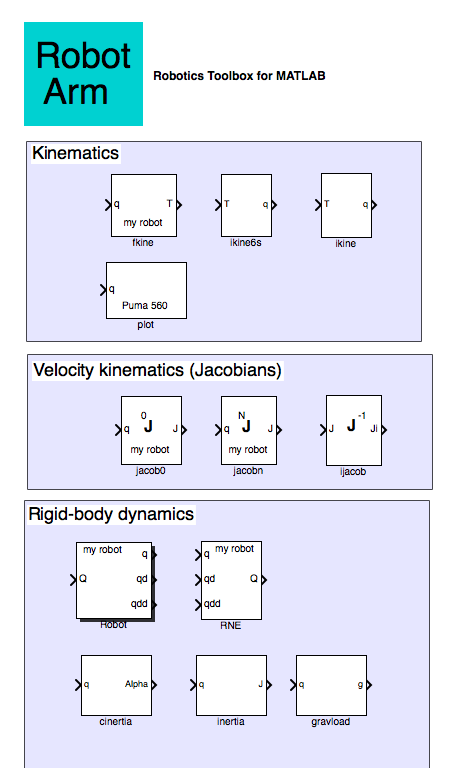
\includegraphics[width=6cm]{figs/roblocks2.png} \\
(a) & (b) 
\end{tabular}
\caption{The Robotics Toolbox blockset.}\label{fig:blockset}
\end{figure}


Simulink\textsuperscript{\textregistered} is the block-diagram-based simulation environment for MATLAB.
It provides a very convenient way to create and visualize complex dynamic
systems, and is particularly applicable to robotics.
RTB includes a library of blocks for use
in constructing robot kinematic and dynamic models.
The block library is opened by
\begin{verbatim}
>> roblocks
\end{verbatim}
and a window like that shown in Figure \ref{fig:blockset}(a) will be displayed.  Double click a particular category and it
will expand into a palette of blocks, like Figure \ref{fig:blockset}(b), that can be dragged into your model.

Users with no previous Simulink experience are advised
to read the relevant Mathworks manuals and experiment with the examples 
supplied.
Experienced Simulink users should find the use of the Robotics blocks quite
straightforward.  Generally there is a one-to-one correspondence between
Simulink blocks and Toolbox functions.
Several demonstrations have been included with the Toolbox in order to 
illustrate common topics in robot control and demonstrate Toolbox Simulink 
usage.
These could be considered as starting points for your own work, just select
the model closest to what you want and start changing it.
Details of the blocks can be found using the File/ShowBrowser option on
the block library window.


% new

\begin{longtable}{p{0.2\textwidth}p{0.75\textwidth}}

Arm robots \\
\texttt{Robot} & represents a robot,  with 
generalized joint force input and joint coordinates, velocities and
accelerations as outputs.
The parameters are the robot object
to be simulated and the initial joint angles.
It is similar to the \texttt{fdyn()}
function and represents the forward dynamics of the robot. \\

\texttt{rne} &  computes the inverse dynamics using
the recursive Newton-Euler algorithm (function \texttt{rne}).
Inputs are joint coordinates, velocities and
accelerations and the output is the generalized joint force.
The robot object is a parameter.\\

\texttt{cinertia} & computes the manipulator Cartesian inertia matrix. The parameters are the robot object
to be simulated and the initial joint angles.\\

\texttt{inertia} & computes the manipulator joint-space inertia matrix. The parameters are the robot object
to be simulated and the initial joint angles.\\

\texttt{inertia} & computes the gravity load. The parameters are the robot object
to be simulated and the initial joint angles.\\

\texttt{jacob0} & outputs a manipulator Jacobian matrix, with respect
to the world frame,  based on the
input joint coordinate vector.
outputs the Jacobian matrix.  
The robot object is a parameter.\\

\texttt{jacobn} & outputs a manipulator Jacobian matrix, with respect
to the end-effector frame,  based on the
input joint coordinate vector.
outputs the Jacobian matrix.  
The robot object is a parameter.\\

\texttt{ijacob} & inverts a Jacobian matrix.  Currently limited
to square Jacobians only, ie. for 6-axis robots.\\

\texttt{fkine} & outputs a homogeneous transformation for the 
pose of the end-effector corresponding to the input joint coordinates.
The robot object is a parameter.\\

\texttt{plot} &  creates a graphical animation of the robot in a new window. The robot object is a parameter.\\

\cmidrule{1-1}
Mobile robots \\

\texttt{Bicycle} & is the kinematic model of a mobile robot that uses the bicycle model. The inputs are speed and steer angle and the outputs are position and orientation. \\
\texttt{Unicycle} & is the kinematic model of a mobile robot that uses the unicycle, or differential steering, model. The inputs are speed and turn raate and the outputs are position and orientation.\\ 

\texttt{Quadrotor} & 
is the dynamic model of a quadrotor. The inputs are rotor speeds and the output is translational and angular position and velocity. Parameter is a quadrotor structure.\\

\texttt{N-rotor} & 
is the dynamic model of a N-rotor flyer. The inputs are rotor speeds and the output is translational and angular position and velocity. Parameter is a quadrotor structure.\\

\texttt{ControlMixer} & accepts thrust and torque commands and outputs rotor speeds for a quadrotor.\\

\texttt{Quadrotor plot} & creates a graphical animation of the quadrotor in a new window.
Parameter is a quadrotor structure.\\

\cmidrule{1-1}
Trajectory \\

\texttt{jtraj} & outputs coordinates of a point following a quintic polynomial as a function of time, as well as its derivatives. Initial and final velocity are assumed to be zero. The parameters include the initial and final points as well as the overall motion time.\\

\texttt{lspb} &outputs coordinates of a point following an LSPB trajectory as a function of time. The parameters include the initial and final points as well as the overall motion time.\\

\texttt{circle} & outputs the xy-coordinates of a point around a circle. Parameters are the centre, radius and angular frequency.\\


\cmidrule{1-1}
Vision \\
\texttt{camera} & input is a camera pose and the output is the coordinates of points projected on the image plane. Parameters are the camera object and the point positions.\\

\texttt{camera2} &input is a camera pose and point coordinate frame pose, and the output is the coordinates of points projected on the image plane. Parameters are the camera object and the point positions relative to the point frame.\\

\texttt{image Jacobian} &input is image points and output is the point feature Jacobian. Parameter is the camera object.\\

\texttt{image Jacobian sphere} &input is image points in spherical coordinates and output is the point feature Jacobian. Parameter is a spherical camera object. computes camera pose from image points. Parameter is the camera object.\\

\texttt{Pose estimation} & computes camera pose from image points. Parameter is the camera object.\\


\cmidrule{1-1}
Miscellaneous \\


\texttt{Inverse} & outputs the inverse of the input matrix.\\

\texttt{Pre multiply} & outputs the input homogeneous transform pre-multiplied by the constant parameter.\\

\texttt{Post multiply} & outputs the input homogeneous transform post-multiplied by the constant parameter.\\

\texttt{inv Jac} & inputs are a square Jacobian $\mathbf{J}$ and a spatial velocity  $\mathbf{\nu}$ and outputs are $\mathbf{J}^{-1}$  and the condition number of $\mathbf{J}$.\\

\texttt{pinv Jac} & inputs are a Jacobian $\mathbf{J}$ and a spatial velocity  $\mathbf{\nu}$ and outputs are $\mathbf{J}^{+}$  and the condition number of $\mathbf{J}$.\\

\texttt{tr2diff} & outputs the difference between two
homogeneous transformations as a 6-vector comprising the translational and
rotational difference.\\

\texttt{xyz2T} & converts a translational vector
to a homogeneous transformation matrix.\\

\texttt{rpy2T} & converts a vector of roll-pitch-yaw angles to
a homogeneous transformation matrix.\\

\texttt{eul2T} & converts a vector of Euler angles to
a homogeneous transformation matrix.\\

\texttt{T2xyz} & converts a homogeneous transformation matrix
to a translational vector.\\

\texttt{T2rpy} & converts a homogeneous transformation matrix
to a vector of roll-pitch-yaw angles.\\

\texttt{T2eul} & converts a homogeneous transformation matrix
to a vector of Euler angles.\\

\texttt{angdiff} & computes the difference between two input angles modulo $2\pi$.
\end{longtable}

A number of models are also provided:

\begin{tabular}{ll}
\cmidrule{1-1}
Robot manipulator arms \\
\texttt{sl\_rrmc} & Resolved-rate motion control  \\
\texttt{sl\_rrmc2} & Resolved-rate motion control (relative) \\
\texttt{sl\_ztorque} & Robot collapsing under gravity \\
\texttt{sl\_jspace} & Joint space control  \\
\texttt{sl\_ctorque} & Computed torque control \\
\texttt{sl\_fforward} &  Torque feedforward control\\
\texttt{sl\_opspace} & Operational space control \\
\texttt{sl\_sea} &  Series-elastic actuator \\
\texttt{vloop\_test} &  Puma 560 velocity loop \\ 
\texttt{ploop\_test} & Puma 560 position loop \\ 
\cmidrule{1-1}
Mobile ground robot\\
\texttt{sl\_braitenberg} &  Braitenberg vehicle moving to a source\\
\texttt{sl\_lanechange} &  Lane changing control \\
\texttt{sl\_drivepoint} &  Drive to a point\\
\texttt{sl\_driveline} &  Drive to a line\\
\texttt{sl\_drivepose} &  Drive to a pose\\
\texttt{sl\_pursuit} &  Drive along a path \\ 
\cmidrule{1-1}
Flying robot\\
\texttt{sl\_quadrotor} &  Quadrotor control \\
\texttt{sl\_quadrotor\_vs} &  Control visual servoing to a target
\end{tabular}


\subsection{Notes on implementation and versions}
The Simulink blocks are implemented in Simulink itself with calls to MATLAB code, or as Level-1 S-functions (a proscribed coding format which MATLAB functions
to  interface with the Simulink simulation engine).

Simulink allows signals to have matrix values but not (yet) object values.  Transformations must be represented as matrices, as per the classic functions, not classes.
Very old versions of Simulink (prior to version 4) could only handle scalar signals which limited its usefulness for robotics.

\subsection{Documentation}
This document {\tt robot.pdf} is a comprehensive manual that describes all functions in the Toolbox.
It is auto-generated from the comments in the \Mlab\ code and is fully hyperlinked:
to external web sites, the table of content to functions, and the ``See also'' functions
to each other.

%The same documentation is available online in
%alphabetical order at \url{http://www.petercorke.com/RTB/r10/html/index_alpha.html}
%or by category at \url{http://www.petercorke.com/RTB/r10/html/index.html}.
%Documentation is also available via the \Mlab\ help browser,  under supplemental software, as ``Robotics
%Toolbox".


\section{Compatible MATLAB versions}
The Toolbox has been tested under R2019b and R2020aPRE.  Compatibility problems are increasingly likely the older your version of \Mlab\ is.

\section{Use in teaching}
This is definitely encouraged!
You are free to put the PDF manual (\texttt{robot.pdf} or the web-based documentation {\texttt{html/*.html} on a server for class
use.
If you plan to distribute paper copies of the PDF manual then every copy must include the first two pages (cover and licence).

Link to other resources such as MOOCs or the Robot Academy can be found at \url{www.petercorke.com/moocs}.

\section{Use in research}
If the Toolbox helps you in your endeavours then I'd appreciate you citing the Toolbox when you publish.
The details are:
\begin{verbatim}
@book{Corke17a,
    Author = {Peter I. Corke},
    Note = {ISBN 978-3-319-54413-7},
    Edition = {Second},
    Publisher = {Springer},
    Title = {Robotics, Vision \& Control: Fundamental Algorithms in {MATLAB}},
    Year = {2017}}
\end{verbatim}
or
\begin{quote}
P.I. Corke, Robotics, Vision \& Control: Fundamental Algorithms in MATLAB. Second edition. Springer, 2017. ISBN 978-3-319-54413-7.
\end{quote}
which is also given in electronic form in the CITATION file.

\section{Support}
There is no support!  This software is made freely available in the hope that you find it useful in solving whatever problems
you have to hand.
I am happy to correspond with people who have found genuine
bugs or deficiencies but my response time can be long and I can't guarantee that I respond to your email.

\textbf{I can guarantee that I will not respond to any requests for help with assignments or homework, no matter
how urgent or important they might be to you.  That's what your teachers, tutors, lecturers and professors are paid to do.}

You might instead like to communicate with other users via 
the Google Group called ``Robotics and Machine Vision Toolbox'' 
\begin{quote}
\url{http://tiny.cc/rvcforum}
\end{quote}
which is a forum for discussion.
You need to signup in order to post, and the signup process is moderated by me so allow a few
days for this to happen.  I need you to write a few words about why you want to join the list
so I can distinguish you from a spammer or a web-bot.

\section{Related software}

\subsection{Robotics System Toolbox\textsuperscript{TM}}
The Robotics System Toolbox\textsuperscript{TM} (RST) from MathWorks is an official and supported product.  System toolboxes (see also the Computer Vision System Toolbox) are aimed at developers of systems. 
RST has a growing set of functions for mobile robots, arm robots, ROS integration and pose representations but its design (classes and functions) and syntax is quite different to RTB.  A number of examples illustrating the use of RST are given in the folder \texttt{RST} as Live Scripts (extension \texttt{.mlx}), but you need to have the  Robotics System Toolbox\textsuperscript{TM} installed in order to use it.

\subsection{Octave}
GNU Octave (www.octave.org) is an impressive piece of free software that implements a language that is close to, but not the same as, \Mlab. The Toolboxes currently do not work well with Octave, though as time goes by compatibility improves.  
Many Toolbox functions work just fine under Octave, but most classes do not.

For uptodate information about running the Toolbox with Octave check out the page \url{http://petercorke.com/wordpress/toolboxes/other-languages}.

\subsection{Machine Vision toolbox}
Machine Vision toolbox (MVTB) for {\Mlab}.  This was described in an article
\begin{verbatim}
@article{Corke05d,
        Author = {P.I. Corke},
        Journal = {IEEE Robotics and Automation Magazine},
        Month = nov,
        Number = {4},
        Pages = {16-25},
        Title = {Machine Vision Toolbox},
        Volume = {12},
        Year = {2005}}
\end{verbatim}
and provides a very wide range of useful computer vision functions and is used to illustrate principals in the Robotics, Vision \& Control book.  You can obtain this from \url{http://www.petercorke.com/vision}.
More recent products such as \Mlab\ Image Processing
Toolbox and \Mlab\ Computer Vision System Toolbox provide functionality that overlaps with MVTB.  

\section{Contributing to the Toolboxes}
I am very happy to accept contributions for inclusion in future versions of the
toolbox.  You will, of course, be suitably acknowledged (see below).

\section{Acknowledgements}
I have corresponded with a great many people via email since the first 
release of this Toolbox.  Some have identified bugs and shortcomings
in the documentation, and even better, some have provided bug fixes and
even new modules, thankyou.  See the file \texttt{CONTRIB} for details.

I would especially like to thank the following. Giorgio Grisetti and Gian Diego Tipaldi for the core of the pose graph solver.
Arturo Gil for allowing me to ship the STL robot models
from \href{http://arvc.umh.es/arte/index_en.html}{ARTE}.
J\"{o}rn Malzahn has donated a considerable amount of code, his
Robot Symbolic Toolbox for MATLAB.
Bryan Moutrie has contributed parts of his open-source package phiWARE to RTB, the remainder of that package can be found online.
%Alexander Lavin has contributed variants of A* and D* planners.
Other special mentions to Gautam Sinha, Wynand Smart for models of industrial robot arm, Pauline Pounds for the quadrotor and related models, 
 Paul Newman for inspiring the mobile robot code, and Giorgio Grissetti for inspiring the pose graph code.


\renewcommand{\section}{\funcsection}
%\setcounter{secnumdepth}{-1}
%\settocdepth{section}
\newpage
\chapter{Functions and classes}
\IfFileExists{all.tex}{\input{all}}{} 

\bibliographystyle{ieeetr}
\bibliography{strings,robot,control,dynamics,kinematics,force,grind,publist,software}
\end{document}
